\chapter{IoT-Device-Management}
\label{sec:devmgmt}
In Zukunft ist eine stark ansteigende Anzahl an IoT-Devices zu erwarten. Laut der International Data Corporation (IDC) dürften im Jahre 2020 in etwa 30 Milliarden Devices weltweit verbunden sein \cite{IDC15}. Unternehmen könnten potenziell mehrere Tausend Sensoren für ihre Zwecke einsetzen. Bereits bei herkömmlichen Computersystemen und Servern stellt das Management eine grosse Herausforderung dar. IoT-Devices dürften potenziell in einer sehr viel grösseren Anzahl verbreitet sein als herkömmliche Geräte. Herausforderungen wie die Heterogenität, Verteilung und Security verschärfen sich mit der stetig wachsenden Anzahl an Geräten. 

IoT-Devices durchleben in ihrem Lebenszyklus verschiedene Stadien. Ein Device-Management Tool soll die Administration in jeder dieser Phasen unterstützen.
\section{Device Lifecycle}
Der Lebenszyklus eines IoT-Devices könnte beispielsweise aus folgenden fünf Phasen bestehen.
\begin{figure}[H]
\centering
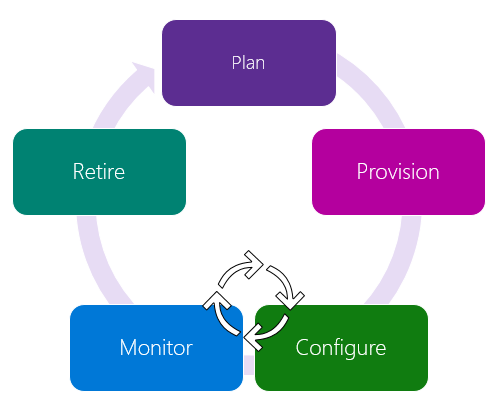
\includegraphics[scale=0.5]{../02_Analyse/images/hubdevmgmt-azure.png}
\caption{IoT-Management Azure \cite{IoTMgmtAzure}}
\end{figure}
\subsubsection{Plan}
In der Planungsphase möchte man aufgrund von vorliegenden Daten eine Veränderung am System vornehmen. Um fundierte Entscheide in der Planungsphase zu ermöglichen werden Daten und Messwerte von Devices benötigt. Je einfacher diese Daten zugänglich-, respektive abfragbar sind, desto qualitativ hochwertiger und exakter kann geplant werden.
\subsubsection{Provision}
Neue Geräte müssen vor der produktiven Nutzung bereitgestellt werden. Dieser Prozess kann mehrere Personen und Aufgaben involvieren. Grundsätzlich werden neue Geräte in ein bestehendes System eingebunden oder ein komplett neues System aufgebaut.
\subsubsection{Configure}
Damit ein Device in den vorgesehenen Zustand versetzt werden kann, benötigt es eine Konfiguration. Bei einer grossen Anzahl Devices empfiehlt es sich diesen Prozess bestmöglichst zu automatisieren. 
\subsubsection{Monitor}
In der Monitoringphase sollen die Zustände der Devices überwacht werden. Ziel ist es, die Funktionalität und Korrektheit des angestrebten Verhaltens sicherzustellen. Dies wird mittels periodischer Abfragen oder Observations sichergestellt. 
\subsubsection{Retire}
Am Ende des Lebenszyklus sollen Geräte geordnet aus dem System entfernt werden. Dabei gilt es den Prozess bestmöglich zu automatisieren und allfällige Vorschriften betreffend Datensicherheit und Datenschutz zu beachten. Andere Systeme wie das Inventar könnten ebenfalls in diesem Prozess beteiligt sein.
\section{Device Management Aufgaben}
\subsection{Provisionierung und Authentisierung}
Bevor neue Devices produktiv genutzt werden können, müssen sie entweder manuell oder automatisch provisioniert werden. Beim Device Provisioning muss ein Gerät in einen Zustand gebracht werden, in dem es für eine oder mehrere vorgesehene Personen erreichbar respektive verfügbar ist.

\subsubsection{Notwendige Schritte}So unterschiedlich die Geräte im Netzwerk und Internet auch sein können, so haben sie abstrakt gesehen die selben Schritte zu durchlaufen um für die produktive Nutzung Verfügbar zu werden:
\begin{itemize}
\item ein Device muss physisch am vorgesehenen Ort platziert werden
\item die Stromversorgung (Stromnetz, Batterie, Akku) für das Gerät muss sichergestellt werden
\item das Device muss gestartet werden
\item eine Initialkonfiguration muss geladen werden
\item die Netzwerk- respektive Internetverbindung muss hergestellt werden
\end{itemize}
Ab dem Zeitpunkt der Erreichbarkeit des Netzwerks unterscheiden sich manuelles und automatisches Provisioning. Beim manuellen Provisioning greift der User oder Administrator entweder direkt über ein grafisches User Interface auf das Gerät zu und nimmt weitere Einstellungen vor oder er verbindet sich über das Netzwerk auf eine Benutzeroberfläche des Geräts. Beim automatischen Provisioning meldet sich das Device über das Netzwerk an einem Controller, respektive einer Management-Instanz.

\subsubsection{Authentisierung} Bei einem Eintritt in ein bestehendes System, in diesem Falle die Bereitstellung eines neuen Devices, muss sich das Gerät am System authentisieren. Aus Sicherheitsgründen möchte man sicherstellen, dass die Zugriffe in das System kontrolliert werden. Es gibt verschiedene Möglichkeiten der Authentisierung:
\begin{itemize}
\item Authentisierung durch Wissen (z.B. Passwort, PIN, Challenge)
\item Authentisierung durch Besitz (z.B. RFID-Chip, Zertifikat, One Time Pin)
\item Authentisierung durch biometrische Merkmale (z.B. Fingerprint, Handvene)
\end{itemize}
Nicht alle Verfahren eignen sich für die Authentisierung von Devices. Ein Gerät selbst verfügt über keine biometrischen Merkmale, höchstens der Benutzer, welcher versucht das Gerät bereitzustellen. Ein Shared Secret in Form eines Passworts oder eine Chain-of-Trust mit Zertifikaten eignen sich für die Device Authentisierung besser. 
\newpage
\subsubsection{IoT-Provisioning} IoT-Devices sollten vor der produktiven Nutzung in einem definierten Prozess bereitgestellt werden. IoT-Devices befinden sich häufig nicht in einer standardisierten Büroumgebung wie zum Beispiel Notebooks und Drucker. Mögliche Standorte sind Lagerhallen, Produktionsstätten oder auch andere Orte im Freien. Oft ist es nicht möglich solche Geräte an das Stromnetz anzuschliessen, deshalb werden diese über Batterien oder einen Akku gespiesen. Die Netzwerk- und Internetverbindung wird über ein Wireless-Mesh-Netzwerk realisiert. In einem ersten Schritt muss ein Device mit einem Netzwerk verbunden werden. Es ist weitgehend bekannt, dass eine grosse Vielfalt an Devices existieren. Manche von ihnen enthalten ein einfaches User Interface, andere nicht. So unterscheidet sich das Ausrollen von IoT-Geräten von herkömmlichen PCs und Laptops indem man nicht direkt über das geräteeigene UI Einstellungen vornehmen kann. Ein Management von IoT-Devices muss also unterschiedliche Anforderungen abdecken. Es könnten sowohl Geräte im herkömmlichen Sinne über eine direkte Internetverbindungen provisioniert werden, als auch neuartige Geräte, welche an ein Low-Power \& Lossy Network (LLN) angeschlossen sind.     

Ein neues IoT-Device im System kontaktiert entweder seinen lokalen Gateway oder direkt einen Server über TCP/IP. Das System kann nun das neue Device aufnehmen und weitere Aufgaben wie beispielsweise das Laden der Konfiguration oder das Speichern von Geräteinformationen veranlassen. Netzwerke mit IoT-Devices sind sehr dynamisch. Es werden häufig neue Teilnehmer aufgenommen oder alte Teilnehmer entfernt. Tools, welche diese Prozesse automatisieren sind stark gefragt. Devices sollen sich selbständig an Netzwerken anmelden können und sich bei zuständigen Servern für weitere Anweisungen registrieren. Solche Discovery Mechanismen sind für zukünftige Anwendungen essentiell \cite{IoTDiscovery10}.

Mit dem Prozess der automatischen Registrierung an Netzwerken und Systemen sind Fragen der Sicherheit verbunden. Man möchte selbstverständlich die Zugriffe in Netzwerke und Systeme korrekt authentisieren und autorisieren. Sicheres Bootstrapping von IoT-Devices umfasst neben Authentisierung und Autorisierung auch die Übertragung von Security Parametern für die Ausführung von vertrauenswürdigen Operationen \cite{IoTSecurityChallenges}.
\subsection{Konfiguration}
\subsubsection{Konfigurationsmanagement} Konfigurationsmanagement beschäftigt sich mit der Erstellung, Verteilung, Versionierung und Sicherung der Konfigurationen von unterschiedlichen Devices. Durch eine Konfiguration wird das Verhalten eines Geräts bestimmt. Die grösste Schwierigkeit bei den Konfigurationen liegt in der Heterogenität. Unterschiedliche Hersteller verwenden für ihre Geräte unterschiedliche Konfigurationen. Selbst Devices derselben Hersteller benötigen oft eine andere Konfiguration. Im Kern lassen sich diese Tatsachen nicht ändern, man kann lediglich versuchen eine möglichst generische Basiskonfiguration für eine Gruppe von Devices bereitzustellen, um die manuellen Tätigkeiten zu minimieren. 

\subsubsection{Automatische Konfiguration} Eine manuelle Konfiguration von sämtlichen IoT-Devices scheint nicht zeitgemäss. So müsste vor jeder Auslieferung das Gerät mit allen Besonderheiten vorinstalliert werden. Stattdessen sollte eine möglichst generische Konfiguration automatisch geladen werden (Zero Touch Provisioning). Bei Bedarf könnte die Konfiguration remote angepasst werden \cite{Weber16}. Auf diese Weise würden beispielsweise in einem WSN von IoT-Devices sämtliche Sensorgeräte initial mit derselben Konfiguration gestartet werden. Möchte man punktuell eine Veränderung an einem Gerät vornehmen, so wäre dies Remote möglich, da mit der generischen Initialkonfiguration Connectivity und Managability sichergestellt würden.
\newpage
\subsubsection{Softwareverteilung} Nebst dem erstmaligen Laden und Anpassen der Konfigurationen von Devices müssen auch deren Soft-, respektive Firmware verwaltet werden. Bei notwendigen Patches und Upgrades sollten diese von Remoteseite aus provisioniert werden können. So können bei bekannt werdenden Sicherheitslücken eine grosse Anzahl Geräte mit Updates versorgt werden. Die Schwierigkeit liegt darin, die möglicherweise grosse Datenmenge der Soft- oder Firmwares auf Geräte in LLNs zu übertragen.

\subsubsection{Backup und Restore} Backup und Restore der Devicekonfigurationen sind wichtige Aufgaben im Device-Management. Die Sicherungsvorgänge müssen entweder automatisch über ein Scheduling, oder manuell von einer Person vorgenommen werden können. Eine manuelle Sicherung ist vor allem bei einer einmaligen Anpassung an der Konfiguration notwendig. 

Die Aufgaben des Konfigurationsmanagements sind immens wichtig. Bei fehlerhaften Konfigurationen oder Ausfällen respektive Defekten von Devices drohen kostspielige Downtimes. Es wäre gar möglich, dass eine ganze Produktionskette für längere Zeit ausfällt. Weitgehend automatisierte Prozesse bei Konfigurationen, sei es das Laden oder das Sichern, stellen einen enormen Mehrwert für den Betrieb von IoT-Devices dar.

\subsection{Monitoring und Diagnose}
\subsubsection{Monitoring allgemein}
Das Hauptziel des Monitorings ist das proaktive Überwachen der Devices. Dadurch verringert sich nicht nur die Zeit, die benötigt wird um den Fehler zu erkennen, sondern auch die benötigte Reparaturzeit. Ein weiteres Ziel ist das Erkennen von Mustern. So können all die gesammelten Daten zusammengefügt- und die Muster analysiert werden, Dies führt zu einer besseren Früherkennung. Zukünftige Probleme können so besser erkannt- und schneller behoben werden
\cite{MonZiele}

\subsubsection{Monitoring im IoT-Bereich}
Im Bereich IoT gibt es spezielle Anforderungen an das Monitoring. Durch die vielen Devices und die dynamischen Netzwerke muss das Monitoring flexibel sein. Täglich werden neue Device eingeführt und alte entsorgt. Nicht nur der Austausch von von Geräten ist mühselig, sondern auch die möglichen Standortwechsel. Die Devices bewegen sich zum Teil und sind so in verschiedenen Netzwerken.

Schlussendlich unterscheidet sich auch die Art der Überwachung. IoT-Monitoring ist nicht mit herkömmlichem Monitoring gleichzustellen. Zum Beispiel bei Serverfarmen sind Auslastung, verfügbarer Speicher wichtig. Bei IoT-Devices sind andere Faktoren wie Verfügbarkeit und Software-Versionen wichtiger. Auch die gewonnen Daten können wichtig sein. Falls zum Beispiel bei Temperaturmessungen arktische Kälte anstelle von sommerlichen Temperaturen gemessen werden, ist das sicher auch ein Indiz für Fehlverhalten.\cite{MonTypes}

\subsection{Maintenance und Update}
\subsubsection{Maintenance und Update Allgemein}
Unter Maintenance versteht man die Wartung und das dazugehörige Updaten der Devices. Bei einer kleinen Anzahl von Geräten funktioniert dies vielleicht noch gut mit einer von Hand geführten Liste, aber bei Hunderten oder gar Tausenden von Geräten wird es schnell unübersichtlich. Daher wird ein Maintanence-Management benötigt.

Ein Bestandteil des Maintenance-Managements ist das Asset-Management. Beim Asset-Management werden alle Gerätedaten, Handbücher, Garantien und andere relevante Daten des entsprechenden Geräts gespeichert.\cite{MainAsset} So hat man eine zentrale Verwaltung aller wichtigen Daten und kann effizienter arbeiten.

Heutige Geräte werden mit einem Softwarestand ausgeliefert, bei denen noch Fehler vorhanden sein könnten. Daher veröffentlichen Gerätehersteller ständig neue Updates und Patches, um neue Funktionen und Sicherheitsupdates einzuspielen. Ohne ein Update-Management wäre diese Aufgabe für so viele Geräte unmöglich. Daher ist eine zentrale Verwaltung unbedingt nötig. 
\subsubsection{Maintenance und Update im IoT-Bereich}
Da es bei IoT-Geräten häufig um Sensoren handelt, welche auch im freien Gelände platziert werden können, ist ein Wartungsmanagement sehr wichtig. Solche Sensoren sind der Umwelt erschwerteren Bedingungen ausgesetzt als normale PCs oder Netzwerkgeräte.

Ohne ein ausgereiftes Management, kann diese Menge aber nicht gewartet werden. So soll das Management eine Empfehlung geben, wann die Batterie auszutauschen ist, oder wann der Sensor nicht mehr die gewünschte Genauigkeit liefert. So weiss der Techniker genau, wann welche Sensoren/Geräte ausgetauscht werden müssen.

Ein weiteres Problem könnten allfällig grosse Distanzen zu Sensoren betragen. Der Sensor befindet sich vielleicht mehrere Kilometer entfernt an schwer erreichbaren Orten.

IoT-Geräte sollte jahrelang im Einsatz sein. Doch Hersteller könnten Konkurs gehen oder pflegen ein Produkt nicht weiter. Nun kann es zum Problem kommen, wenn ein Sensor keine Updates mehr erhält und schwerwiegende Sicherheitslücken vorhanden sind, vor solchen Szenarien sollte man gewarnt werden. 

Durch die vielen Software Updates bei der hohen Anzahl an Geräten, ist man ohne automatische Softwareverteilung überfordert. Von Hand kann diese hohe Anzahl an Geräte kaum bewältigt werden. Mit einer Softwareverteilung würde man den gewünschten Softwarestand freigeben, die Managementumgebung verteilt diese automatisch auf die jeweiligen Sensoren. Bei Problemen wird der Administrator benachrichtigt und kann eingreifen.

Bei der grossen Anzahl von Updates darf das Netzwerk nicht vernachlässigen werden. Bedenkt man, dass IoT-Netzwerke für geringere Bandbreite ausgelegt sind, muss unbedient auf die Datenmenge geachtet werden. Bei vielen Geräten könnte ein solches Netzwerk überlastet werden wenn man allen Geräten gleichzeitig ein Update schickt.
